\section{Experimental results}\label{sec:experiments}

In this section, we provide an experimental evaluation of our approach
based on two classes of test instances. More precisely, we test our approach on the following MDPS:
\begin{itemize}
\item Random MDPs (\texttt{Random}).
\item Diamond MDPs (\texttt{Diamond}).
\item Grid MDPs (\texttt{Grid}).
\end{itemize}


For each class of MDP, we provide a brief description of its structure and of the parameters used to generate the testbed.

As already mentioned in the introduction, the aim of this section is two-fold:

(i) First of all, we would like to motivate the use of deterministic over stochastic policies. To do this, we compare the value of the maximum regret obtained by the optimal deterministic policy with the one of the rounding policy explained in Section~\ref{sec:rounding}. 
%
%The TUP uses the concept of sparsity presented in this paper to generalize the methodology proposed in~\cite{Buchheim18} to solve efficiently combinatorial problems with a quadratic objective function.
%In Section~\ref{sec:TUP} we show how the application of TUD allows to improve the dual bounds obtained in the approach presented in~\cite{Buchheim18}.  

(ii) Secondly, we would like to assess the additional computational effort of computing the optimal deterministic policy in comparison to the one needed to compute the optimal stochastic policy. 	 

In the following section we use the notion of Time ratio ($TR$) and Value Ratio ($VR$), defined as follows:

\begin{definition}
For a given MDP, let $MR(f^{\hat{\pi}}, \mathcal{R})$ be the maximum regret of the rounding deterministic policy and $MR(f^{\pi^*}, \mathcal{R})$  be the maximum regret of the optimal deterministic policy. We have that the Value Ratio of such MDPs is defined as follows:
\begin{align}
VR = \dfrac{MR(f^{\hat{\pi}}, \mathcal{R})}{MR(f^{\pi^*}, \mathcal{R})}\;.
\end{align} 
Moreover, let $\hat{T}$ (respectively $T^*$) be the computing time necessary to calculate the rounding (respectively optimal) deterministic policy, we have that the Time Ratio is defined as:
\begin{align}
TR=\dfrac{T^*}{\hat{T}}\;.
\end{align}
 
\end{definition}

\subsection{Random MDPs}
\paragraph{Description}
A random MDP is defined by several parameters including its number of states $n$ , its number of actions $k$. All rewards are bounded between randomly two real numerical points. Transition function has several properties: from any state $s$ restrict transitions to reach $\lceil \log_2(n) \rceil$ states. For each pair of $(s, a)$ draw reachable states based on uniform
distribution over the set of states. For drawn states, transition probabilities are formed based on Gaussian distribution.
The initial state distribution β is uniform and we choose discount factor $\gamma = 0.95$. 
\paragraph{Analysis of the results}
In Table~\ref{tab:random} we have th resutm

\begin{table}[h] % <-- HERE
 \setlength{\tabcolsep}{2.5pt}
 \renewcommand \arraystretch{1.1}
\begin{center}
\begin{tabular}{rrrrrrrrrrrrrrrrrrrrrrrrrrrr}
	&		&				&				&				&	\multicolumn{2}{c}{	\texttt{Comp. Time}}	\\
$|S|$	&	$|A|$	&		\texttt{VR}		&		\texttt{TR}		&		\texttt{\% diff}		&	\texttt{Base}	&	\texttt{C\&B}	\\
\cmidrule(lr){1-2} \cmidrule(lr){3-3} \cmidrule(lr){4-4}  \cmidrule(lr){5-5}  \cmidrule(lr){6-7}
5	&	2	&			1.07	&			1.83	&			50\%	&	2.59	&	2.27	\\
	&	3	&			1.03	&			2.44	&			20\%	&	5.05	&	5.11	\\
	&	4	&			1.09	&			2.17	&			50\%	&	5.28	&	4.67	\\
	&	5	&			1.07	&			2.85	&			50\%	&	8.03	&	7.99	\\
	&	10	&			1.02	&			2.50	&			30\%	&	13.76	&	12.61	\\
\cmidrule(lr){1-2} \cmidrule(lr){3-3} \cmidrule(lr){4-4}  \cmidrule(lr){5-5}  \cmidrule(lr){6-7}
10	&	2	&			1.11	&			4.11	&			90\%	&	21.78	&	20.12	\\
	&	3	&			1.15	&			7.63	&			80\%	&	81.67	&	73.43	\\
	&	4	&			1.04	&			9.19	&			60\%	&	312.05	&	266.35	\\
	&	5	&			1.06	&			8.42	&			90\%	&	570.15	&	478.07	\\
	&	10	&			1.01	&			18.79	&			90\%	&	1886.05	&	986.71	\\
\cmidrule(lr){1-2} \cmidrule(lr){3-3} \cmidrule(lr){4-4}  \cmidrule(lr){5-5}  \cmidrule(lr){6-7}
15	&	2	&			1.04	&			6.91	&			60\%	&	94.95	&	82.59	\\
	&	3	&			1.05	&			18.75	&			80\%	&	2240.40	&	2024.85	\\
	&	4	&			1.01	&			20.04	&			80\%	&	5366.92	&	3181.01	\\
	&	5	&			1.03	&			32.10	&			100\%	&	7677.25	&	4127.52	\\
\cmidrule(lr){1-2} \cmidrule(lr){3-3} \cmidrule(lr){4-4}  \cmidrule(lr){5-5}  \cmidrule(lr){6-7}
	&	Avg.	&			1.06	&			7.77	&			70\%	&	1306.14	&	805.24	
\end{tabular}						
\end{center}
\caption{Time Ratio and Value Ratio for \texttt{Random} MDPs.}														\label{tab:random}								
\end{table} % <-- HERE



\subsection{Diamond MDPs}
\paragraph{Description}
This class of MDPs has been introduced for the first time in~\cite{benavent2018}. 
In this family of problems the reward of a few states suffices to generate a lot of uncertainty about the optimal policy. This class of instances is an interesting set of instancess to test our proposed algorithm.
This class of MDPs has a diamond structure, with one top and one bottom state (playing the role of source and sink of the  MDP), one intermediate layer of states, containing all the uncertainty in the reward, plus two intermediate layer between the extrem states and the intermediate layer.
In Figure~\ref{fig:diamond}, the structure of the diamond MDPs is presented.

\begin{figure}[h]
\begin{center}
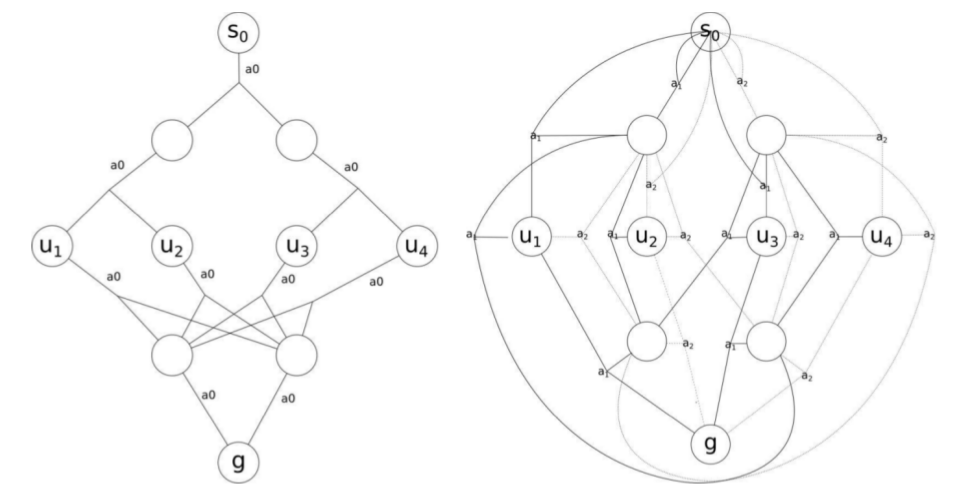
\includegraphics[width=8cm]{images/diamond.png}
\end{center}
\caption{Diamond MDP: actions $a_0$ (left) and $a_1, a_2$ (right).}
\label{fig:diamond}
\end{figure}

From a point of viex of the parameters, the authors proposed to have that action $a_0$ would reach each child with a probability of $0.5$. ON the other hand $a_1$ (resp. $a_2$) a probability of $p= 0.3$ (resp. $1-0.3$) to reach the left (resp. right) child node and to reach its parent otherwise.
The imprecise values of the rewards for the middle layer are $[-600,600]$, while the one of the bottom node is $[600,1000]$.

We propose a generalization of this family of MDP in two senses: we test a range of parameters for the probability $p \in \{5,10,\dots,40,45\}$ and we introduce also an additional intermediate layer, between the extreme states and the middle layer. In this way we have, in addition to $10$-states MDPs (callend one-level diamond MDPs) also  22-states MDPs (called two-level diamond MDPs). 

\paragraph{Analysis of the results}
In Table~\ref{tab:diamond} We show


\begin{table}[h]																	
 \centering
 \small
 \setlength{\tabcolsep}{4.0pt}
 \renewcommand \arraystretch{1.8}
\begin{tabular}{ccccccccccc}																						
p	&	5	&	10	&	15	&	20	&	25	&	30	&	35	&	40	&	45	&	Avg.	\\	
\cmidrule(lr){1-1} \cmidrule(lr){2-10} \cmidrule(lr){11-11}
VR &	1.66	&	1.24	&	1.16	&	1.13	&	1.15	&	1.15	&	1.15	&	1.14	&	1.16	&	\textbf{1.22}	\\	
TR &	10.23	&	7.44	&	6.32	&	6.48	&	7.67	&	5.93	&	7.62	&	10.46	&	13.80	&	\textbf{8.44}	\\	\\
\end{tabular}
\caption{Time Ratio and Value Ratio for \texttt{Diamond}.}														\label{tab:diamond}								
\end{table}																						



\subsection{Grid MDPs}
blablabla
\paragraph{Description}
blablabla
\paragraph{Analysis of the results}
blablabla



\paragraph{Analysis of the Diamond MDPs}

